
\chapter[Teoría de Drude y Sommerfeld]{Teoría de drude y teoría de Sommerfeld para metales} \label{Ch:06}

En este capítulo vamos a tratar dos teorías de los electrones compatibles entre sí: la teoría de Drude de los electrones, que nos permite calcular valores como la conductividad eléctrica, coeficiente de Hall, efecto Peltier... es decir, fenómenos que dependen del movimiento de los electrones en el metal. Por otro lado tendremos la teoría de los electrones libres, que nos permite calcular valores como el coeficiente calorífico, energía interna... es decir, propiedades más relacionadas con la mecánica estadística. A diferencia del manual de la asignatura \cite{Fisica_del_Estado_Solido} nosotros usaremos el \cite{Oxford_Solid_State}, salvo en aquellos puntos que el primero sea mas completo.

\section{Teoría de Sommerfeld o de electrones libres}

En 1925 Pauli descubrió lo que hoy llamamos \textit{principio de exclusión}, que dice que dos electrones no pueden estar en el mismo estado. En 1926, Fermi y Dirac derivaron lo que hoy llamamos estadística de Fermi-Dirac, que permite describir el número y densidad de estados ocupados por fermiones (partículas regidas por el principio de exclusión) a temperatura finitas. Sommerfeld fue quien dió cuenta de que usando la estadística Fermi-Dirac era capaz de describir correctamente el comportamiento del electrón en los metales (incorporando además la Teoría de Drude derivada 30 años antes).

\subsection{Niveles de energía}

El comportamiento de los electrones viene determinado por la función de ondas del mismo, obtenida (a no ser que las energías de estos sean ultrarrelativistas)  mediante la ecuación de Schrödinger:

\begin{equation}
	\parentesis{-\frac{\hbar^2}{2m} \nabla^2 + V(\rn)} \Psi = i \hbar \parciales{\Psi}{t}
\end{equation}
Si tomamos que $\Psi (\rn,t)=e^{-iEt/\hbar} \Psi (\rn)$ donde $E$ es la energía del estado tenemos que la ecuación se transforma en la llamada \textit{ecuación de Schrödinger independiente del tiempo}

\begin{equation}
	\parentesis{-\frac{\hbar^2}{2m} \nabla^2 + V(\rn)} \Psi (\rn) = E \Psi (\rn)
\end{equation}
En función del potencial que usemos para describir el comportamiento de los electrones obtendremos una teoría u otra. La \textit{teoría de los electrones libres} es la mas sencilla de todas, ya que supone que $V(\rn) = 0$, es decir, que los electrones no experimentan ningún tipo de potencial en el metal (ni con otros electrones, ni vibraciones, ni con los átomos...). Es evidente que una teoría que quisiera ser más realista debería incluir algún tipo de potencial, pero como veremos es suficiente como para predecir algunos valores experimentales (aunque sea en orden de magnitud). En ese caso la ecuación se transforma en:

\begin{equation}
	-\frac{\hbar^2}{2m} \nabla^2  \Psi (\rn) = E \Psi (\rn) \label{Ec:06-01-03}
\end{equation}
Que como podemos ver no es más que una ecuación de onda, por lo que la solución mas general puede ser descrita en función de exponenciales complejas

\begin{equation}
	\Psi (\rn) = A e^{i \kn \cdot \rn}
\end{equation}
donde $\kn$ es el vector de onda que debe verificar que:

\begin{equation}
	k^2 = \frac{2mE}{\hbar^2}
\end{equation}
Esta solución, aunque viola los principios de la mecánica cuántica (la integral en el el espacio de $|\Psi|^2$ es infinita, teniendo que ser 1) y no describe estados reales (energía y momento perfectamente definidos, partícula que podría estar en cualquier parte del universo con la misma probabilidad...), es bastante funcional. Si ahora al electrón lo encerramos en una caja de volumen $V=L_xL_yL_z$ y exigimos que la función de ondas sea igual en todo el borde $\Psi (0)=\Psi(L_i)$ ($i=x,y,z$) tenemos que el momento se discretiza (ya no todos los valores son iguales), tal que:

\begin{equation}
	k_i = \frac{2\pi}{L_i} n_i \tquad n_i = 1,2,3\ldots
\end{equation}
para $i=x,y,z$. Supongamos de ahora en adelante que los 3 lados son iguales y que por tanto $V=L^3$. Como podemos ver esto significa que a un $\kn_n$ concreto se le asocia un volumen en el espacio de los momentos $k$ de volumen $8\pi^3 /L^3$. En realidad a cada uno de estos volumenes podremos asociar dos estados de electron: uno con espín $\uparrow$ y otro con espín $\downarrow$. De este hecho podemos obtener un valor para el número de estados posibles $\Ncal$ encerrados en una esfera de radio $k_F$ en el espacio de momentos:

\begin{equation}
	\Ncal = 2 \times \frac{1}{8\pi^3/L^3} \iint_0^{k_F} k_F^2 \D k \D \Omega
\end{equation}
En palabras esta ecuación se traduce como: el número de estados totales para dicha esfera es el volumen de la esfera entre el volumen al que asociamos un estado posible. De este modo tenemos que:

\begin{equation}
	\Ncal = \frac{V}{3\pi^2} k_F^3
\end{equation}
En el cero absoluto, los electrones tratarán de colocarse en los niveles con menos energía posible (es decir, con menor $k$), por lo que si en tenemos $N$ partículas posibles (es decir, tenemos que asignar $N$ estados posibles, tal que $\Ncal \rightarrow N$ en la ec. anterior). Así el valor de $k_F$ adquiere el significado de ``máximo valor posible de $k$ para un electrón'', y tiene el valor de:

\begin{mybox}
\begin{equation}
	k_F =  \parentesis{3\pi^2 n}^{1/3}
\end{equation}
\end{mybox}
donde $n=N/V$ es la \textit{densidad de partículas}. Lógicamente valores de $k>k_F$ no son posibles, ya que eso significaría que esa partícula tiene disponible un estado con menor energía que no está ocupando, lo cual es imposible si estamos en el cero absoluto. Entonces la superficie de la esfera citada antes adquiere un significado más profundo, ya que es la separación entre \textit{los estados ocupados y desocupados} del sistema, denominándose \textbf{superficie de Fermi}. De aquí podemos deducir otros muchos términos (como la energía máxima, velocidad máxima...). A todos estos términos los llamamos ``de Fermi''. Así tenemos, en resumen:

\begin{itemize}
	\item \textbf{Vector de onda de Fermi (3D):}
	\begin{equation}
		k_F = (3\pi^2 n)^{1/3} \quad (n\equiv N/V) \label{Ec:06-01-05}
	\end{equation}
	\item \textbf{Vector de onda de Fermi (2D):}
	\begin{equation}
		k_F= \sqrt{2\pi n}
	\end{equation}
	\item \textbf{Energía de Fermi:}
	\begin{eqnarray}
		\varepsilon_F \equiv \frac{\hbar^2 k_F^2}{2m} \label{Ec:06-01-07}
	\end{eqnarray}
	\item \textbf{Velocidad de Fermi:}
	\begin{eqnarray}
		v_F \equiv \sqrt{2\varepsilon_F /m} \label{Ec:06-01-08}
	\end{eqnarray}
	\item \textbf{Temperatura de Fermi:}
	\begin{eqnarray}
		T_F \equiv \varepsilon_F / k_B
	\end{eqnarray}
\end{itemize}
Ahora otra pregunta que nos podemos hacer es: ¿Cuantos estados hay en un intervalo de energías $\varepsilon$ y $\varepsilon+\D \varepsilon$? Para calcularlos esto solo tenemos que saber cuantos estados hay entre $k$ y $K+\D k$ y hacer el cambio de variable. Entonces en un intervalo $\varepsilon$ y $\varepsilon+\D \varepsilon$ habrá 

\begin{equation*}
	\Ncal (k+\D k) - \Ncal (k) = \frac{V}{3\pi^2} \parentesis{\frac{2m}{\hbar^2}}^{3/2} \parentesis{(\varepsilon+\D \varepsilon)^{3/2} - (\varepsilon)^{3/2} }
\end{equation*}
si ahora $\D \varepsilon \rightarrow 0$ tal que $\Ncal (k+\D k) - \Ncal (k) = \D \Ncal$ tenemos que 

\begin{equation*}
	\D \Ncal = \frac{V}{3\pi^2}\parentesis{\frac{2m}{\hbar^2}}^{3/2} \parentesis{(\varepsilon+\D \varepsilon)^{3/2} - (\varepsilon)^{3/2} } = \frac{V}{3\pi^2} \varepsilon^{3/2} \parentesis{(1+\D \varepsilon/\varepsilon)^{3/2} - (1)^{3/2} } 
\end{equation*}
donde hemos usado que $\sqrt{1+x}\approx 1+x/2$ y cogido el término lineal con $\D \varepsilon$, de tal modo que:

\begin{equation}
	\D \Ncal =\parentesis{\frac{2m}{\hbar^2}}^{3/2} \frac{ \varepsilon^{3/2} V}{3\pi^2}\frac{3}{2} \frac{\D \varepsilon}{\varepsilon}
\end{equation}
Si definimos la \textbf{densidad de estados} como $D(\varepsilon) = \D \Ncal / \D \varepsilon$ tenemos que:
\begin{mybox}
\begin{equation}
	D(\varepsilon) = \frac{V}{2\pi^2} \parentesis{\frac{2m}{\hbar^2}}^{3/2} \varepsilon^{1/ 2}
\end{equation}
\end{mybox}
Teniendo en cuenta que $2m/\hbar^2 = k_F^2 / \varepsilon_F$, y que $k_F=(3\pi^2 n)^{1/3}$ tenemos que la densidad de estados se puede escribir como

\begin{equation}
	D(\varepsilon)  = \frac{3}{2}  \frac{N}{\varepsilon_F} \parentesis{\frac{\varepsilon}{\varepsilon_F}}^{1/2}
\end{equation}
De lo que se puede deducir la expresión de densidad de estados por unidad de volumen $d(\varepsilon)=D(\varepsilon)/V$. Teniendo en cuenta todo lo anterior no es muy difícil deducir que:

\begin{equation}
	N = \int_{0}^{\varepsilon_F} D(\varepsilon) \D \varepsilon
\end{equation}
que sólo es válido para temperaturas $T=0$, ya que estamos asumiendo que la probabilidad de que el estado con $\varepsilon<\varepsilon_k$ esté ocupado es del 100\%. Sin embargo a temperaturas finitas esta probabilidad dependerá de una función llamada la función de Fermi, que como veremos en el siguiente apartado modificará sustancialmente esta ecuación. 

\subsection{Estadística de Fermi-Dirac}

Dado un sistema de electrones libres (es decir, no están sometidos bajo ningún tipo de potencial), la probabilidad de que un estado con energía $E$ esté ocupado viene dado por el factor de Fermi, también llamado \textbf{distribución de Fermi-Dirac}:
\begin{mybox}\begin{equation}
	f_{FD} (E,T) = \dfrac{1}{e^{(E-\mu)/k_BT}-1}
\end{equation}\end{mybox}
donde $\mu$ es el llamado \textit{potencial químico}, aunque en realidad la razón por la cual aparece en la ecuación es en candidad de constante de integración, de multiplicador de lagrange fruto de la derivación matemática. A bajas energías la función de Fermi se convierte en la función escalón, mientras que a altas temperaturas esta función escalón se va difundiendo. Como podremos ver esta estará relacionada con la energía de Fermi.

\begin{figure}[h!] \centering
	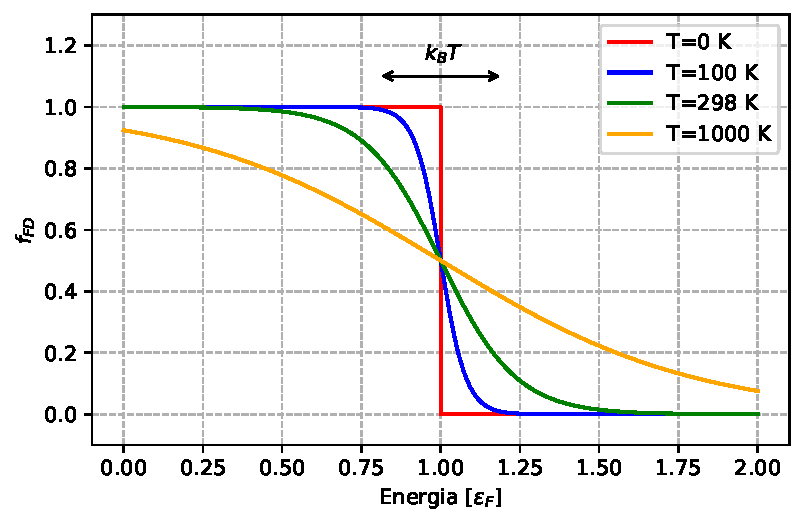
\includegraphics[scale=0.85]{Cuerpo/Ch_06/06-Fermi-Dirac.pdf}
	\caption{Distribución de Fermi-Dirac.}
	\label{Fig:06-0}
\end{figure}    
Cuando $T\neq0$ la probabilidad de que este ocupado un estado de energía $\varepsilon>\varepsilon_F$ ya no es cero, de tal modo que el número de estados viene dado por:

\begin{equation}
	N=\int_{0}^{\infty} f_{FD}(\varepsilon,T) D(\varepsilon) \D \varepsilon \label{Ec:06-01-00}
\end{equation}
Si $T=0$ tenemos que la ecuación () se recupera verificándose que $\mu=\varepsilon_F$ dadas las definiciones previas. Sin embargo para temperaturas $T\neq 0$ no se verifica que sean iguales ($\mu(T\neq 0) \neq \varepsilon_F$). De hecho el valor de $\mu$ depende en última instancia de la ligadura (\ref{Ec:06-01-00}), de tal modo que para $T\ll T_F$ se verifica que:

\begin{equation}
	\mu(T) \approx \varepsilon_F \ccorchetes{1-\frac{1}{3}\parentesis{\frac{\pi T}{2T_F}}^2}
\end{equation}
que se deduce de la expansión de Sommerfeld que veremos en el siguiente apartado.

\section{Energía interna y capacidad calorífica}

El valor de la energía interna de los electrones es bien sencillo de calcular, ya que vendrá dado por la integral

\begin{equation}
	U(T) = \int_0^{\infty} \varepsilon D(\varepsilon) f_{FD} (T,\varepsilon) \D \varepsilon  
\end{equation}
Lo cual es evidente si pensamos en el significado de cada uno de los miembros: la energía total será la suma (integral)  de la energía de cada estado por la probabilidad de que esté ocupado por la cantidad de estados de esa energía. Una vez tenemos esto solo queda calcular la integral. Por ejemplo para $T=0$K tenemos que:

\begin{equation}
	U(0) = \int_0^{\varepsilon_F} \varepsilon D (\varepsilon) \D \varepsilon = \frac{3}{5} N \varepsilon_F
\end{equation} 
Ahora bien: ¿Cual es el valor para $T\neq 0$K? La respuesta está en la integral, pero debido a la forma de $f_{FD}$ no parece que la integral sea sencilla de obtener. La mejor manera de calcular esto es usar la \textit{expansión de Sommerfeld} (que exige $T\ll T_F$), que nos dice que para cualquier función $H(\varepsilon)$ tenemos:

\begin{equation}
	\int_0^{\infty} H(\varepsilon) f_{FD} (\varepsilon) \D \varepsilon \approx 
	\int_0^{\mu} H(\varepsilon) \D \varepsilon + \frac{\pi^2k_B^2T^2}{6} \parentesis{\derivadas{H(\varepsilon)}{\varepsilon}}_{\varepsilon=\mu}
\end{equation}
Así tenemos que la energía total a temperaturas no nulas pero muy inferiores al a temperatura de Fermi:

\begin{equation}
	U(T) = U(0) + \frac{\pi^2}{6} \frac{3 N}{2 \varepsilon_F} k_B^2 T^2
\end{equation}
o lo que es lo mismo:

\begin{mybox}
\begin{equation}
	U(T) = U(0) + \frac{\pi^2}{6} \frac{3 N k_B }{2 } \frac{T^2}{T_F}
\end{equation}
\end{mybox}
De lo que se deduce que la capacidad calorífica debida a los electrones libres  $C_{el} = \parentesis{\partial U/\partial T}_V$ viene dada por

\begin{equation}
	C_{el} = \frac{\pi^2 N}{2} \frac{k_B T}{T_F}
\end{equation}
Es decir, la capcidad calorífica debida a los electrones libres en los metales a bajas temperaturas es típicamente lineal, lo cual no es del todo incorrecto, aunque es cierto que los calores específicos resultantes de esta teoría difieren en un factor 10 respecto al experimental. Lógicamente esto es de esperar, ya que realmente los electrones en los metales no son libres. En general solemos denotar $C_{el} = \gamma T$, de tal forma que:

\begin{equation}
	\gamma = \frac{\pi^2 N}{2} \frac{k_B}{T_F}
\end{equation}
Así tenemos que la capacidad calorífica total a bajas temperaturas
\begin{mybox}
\begin{equation}
	C=C_{el}+C_{fon}= \gamma T + \alpha T^3
\end{equation}
\end{mybox}
lo que hace realmente difícil de medir $\gamma$ experimentalmente, ya que hace falta energías muy bajas para que no predomine la capacidad calorífica fonónica.

\begin{table}[h!] \centering
	\begin{tabular}{cccc} 
		Elemento & $\gamma_{\text{el.libres}}$ &  $\gamma_{\text{exp}}$ & cociente \\
		& $\parentesis{10^{-4} \frac{\text{cal}}{\text{mol}\cdot\text{K}^2}}$& $\parentesis{10^{-4} \frac{\text{cal}}{\text{mol}\cdot\text{K}^2}}$  &  \\ \hline
		Li & 1.8 & 4.2 & 2.3 \\
		Na & 2.6 & 3.5 & 1.3 \\
		Cs & 5.3 & 7.7 & 1.5 \\
		Cu & 1.2 & 1.6 & 1.3 \\
		Au & 1.5 & 1.6 & 1.1 \\
		Sr & 4.3 & 8.7 & 2.0 \\
		Fe & 1.5 & 12 & 8.0 \\
		Zn & 1.8 & 1.4 & 0.78 \\
		Pb & 3.6 & 7.0 & 1.9 \\
		Bi & 4.3 & 0.2 & 0.047 
	\end{tabular}	
	\caption{Predicción de la teoría de $e^-$ libres y resultado experimental para el coeficiente $\gamma$ de distintos elementos.}
	\label{Tab:06-01}
\end{table}

\section{Tratamiento clásico de electrones: tería de Drude}

Los otros metales se caracterizan por una alta conductividad eléctrica, $\sigma$, comparada con otros materiales [$10^8$-$10^7$ ($\Omega$m)$^{-1}$ frente a $10^5$-$10^{-4}$ ($\Omega$m)$^{-1}$ en semiconductores y hasta $10^{-16}$ ($\Omega$m)$^{-1}$ en aislantes]. Electrones completamente libres e independientes (es decir, no interaccionantes con la red o entre ellos) darían lugar a una conductividad eléctrica infinita. Se introduce por tanto un modelo cinético similar al utilizado en el capítulo \ref{Ch:05} con fonones. En este modelo cinético los electrones se tratan clásicamente. Esto es posible porque podemos formar, a partir de las funciones de onda (\ref{Ec:06-01-03}), un paquete de ondas de extensión espacial $\Delta x$ verificando $\Delta k \Delta x \sim 1$. Como $\Delta k$ debe estar bien definido, es decir $\Delta k \ll k_F \sim a^{-1}$, debe ser $\Delta x \gg a$. Por tanto, el modelo será aplicable siempre que las características de posibles perturbaciones (la longitud de onda de campos aplicados o el recorrido libre medio, ver más abajo) sean mucho mayores que $a$. Veamos entonces un poco en que consiste la teoría de Drude.

\subsection{Teoría de Drude}

Desde que J.J. Thomson descubrió en 1896 el electrón, diversos físicos se preguntaron como se movían estas cargas dentro del metal. Fue en 1900 cuando Paul Drude dio cuenta de que aplicando la teoría cinética de los gases de Boltzmann al caso de los electrones en un metal podía describir correctamente su movimiento, siendo así la primera teoría que permitía entender la conducción metálica (aún con sus fallas). La teoría de Drude hace entonces 3 suposiciones básicas:

\begin{itemize}
	\item Existe un tiempo entre las diferentes colisiones\footnote{En la teoría cinética de los gases una colisión se entiende como el choque de las partículas (como dos bolas de billar), sin embargo los electrones interaccionan a través del potencial de Coulomb, que al ser de largo alcance hace difícil estimar una sección eficaz. Además existen otros elementos que pueden interaccionar con los electrones: fotones, fonones, defectos... Por esta misma razón estimar $\tau$ para los electrones es mucho más complicado que estimarlo para los átomos/moléculas de un gas. De hecho suelen interactuar más con fonones y con defectos que con otros electrones.} de electrones $\tau$. La probabilidad de que se haya producido la colisión en un intervalo de tiempo $\D t$ es $\D t /\tau$. 
	\item Una vez ocurre la colisión, asumimos que el momento del electrón se reduce a cero $\pn=0$.
	\item Entre las colisiones, los electrones con carga $-e$, interactuan con los campos externos $\En$ y $\Bn$.
\end{itemize}

Las primeras dos suposiciones son exactamente las mismas que la teoría cinética de gases\footnote{Lógicamente este no es un modelo perfecto, y se podría hacer mucho más realista considerando que en cada colisión las dos partículas iniciales comienzan con momento $\pn_1^{\inicial}$ y $\pn_2^{\inicial}$ y salen con momentos $\pn_1^{\final}$ y $\pn_2^{\final}$ de tal manera que se conserva energía y momento. Desafortunadamente esto hace extremadamente difícil el cálculo, así que veamos cuán incorrectas son las suposiciones hechas. La primera conjetura no está totalmente errada, ya que experimentalmente si se observa un tiempo medio entre colisiones. La segunda si que es mucho más cuestionable, aunque \textit{en promedio} si se verifica  que el momento final es cero. Sin embargo no es correcto que \textit{cada} partícula tenga una energía cinética cero tras la colisión.}. La tercera suposición es una generalización lógica, ya que a diferencia de las moléculas del gas, los electrones están cargados, y por tanto deben interactuar los campos electromagnéticos.

\subsection{Ecuación dinámica de Drude}

Entonces consideremos un electrón con momento $\pn$ en el instante temporal $t$. ¿Cuál será el valor del momento en el instante $t+\D t$? Existe dos términos que influyen en el valor final. El primero es que hay una probabilidad de $\d t/\tau$ de que el momento se haga cero. Si no se hace cero (la probabilidad de que no sea cero es $1-\D t / \tau$) el momento se irá acelerando debido a la fuerza $\Fn$ (en nuestro caso la fuerza generada por los campos electromagnéticos), por lo que el momento en este caso será la suma del momento anterior y el valor $\Fn(t)\D t$. Así, el valor medio del momento en $t+\D t$ será la probabilidad de que se vaya a cero por cero más la probabilidad de que no sea cero mas esta aceleración:

\begin{equation}
	\langle \pn (t + \D t) \rangle = \parentesis{1- \frac{\D t}{\tau}} \parentesis{\pn (t)+\Fn \D t} + \mathbf{0} \D t / \tau
\end{equation}
Manteniendo los términos de primer orden con $\D t$ tenemos la \textbf{ecuación dinámica de Drude}\footnote{Cuando escribimos $\pn$ hablamos del valor medio $\langle \pn \rangle$. Dado que nuestro estudio es puramente probabilístico, deberíamos escribir todas las cantidades como valores medios (hasta la fuerza) de estos eventos aleatorios. Una teoría más detallada debería hablar de ``distribuciones de momento'' mas que de momento medio. Llevando esto a la práctica obtendremos las ecuaciones de transporte de Maxwell, no discutidas aquí.}

\begin{mybox}
\begin{equation}
	\derivadas{\pn}{t} = \Fn - \frac{\pn}{\tau}
\end{equation}
\end{mybox}
donde $\Fn$ es la fuerza que experimenta el electrón, siendo esta la conocida \textit{fuerza de Lorentz}. 

\begin{equation}
	\Fn = - e \parentesis{\Encal + \vn \times \Bn}
\end{equation}
Uno puede considerar al término $\pn/\tau$ coomo una \textit{fuerza de arrastre}. Nótese que en el caso de que no hubiera fuerza de arrastre la ecuación diferencial nos lleva directamente a un decaimiento exponencial del momento:

\begin{equation}
	\pn (t) = \pn_\inicial e^{-t/\tau}
\end{equation}
lo cual es de esperar teniendo en cuenta que las partículas pierden momento con cada colisión.



\section{Electrones en campos externos}

\subsection{Electrones en un campo eléctrico y conductividad eléctrica}

Consideremos entonces que nuestros electrones están ante la presencia de un campo eléctrico no nulo. Entonces nuestra ecuación del movimiento es:

\begin{equation}
	\derivadas{\pn}{t} = -e \Encal - \frac{\pn}{\tau}
\end{equation}
En un estado estacionario tendremos que el momento $\D \pn / \D t = 0$, por lo que

\begin{equation}
	m \vn = \pn = - e \tau \Encal
\end{equation}
siendo $m$ la masa de un electrón y $\vn$ su velocidad (promediada). Como sabemos el podemos relacionar la existencia de un promedio de la velocidad y el flujo de carga. Si $n$ es la densidad de electrones en el metal, $-e$ la carga del electrón y $\vn$ su velocidad, tenemos que el flujo eléctrico es:

\begin{equation}
	\jn = - e n \vn  = \frac{e^2 \tau n}{m} \Encal
\end{equation}
Como podemos observar $\jn$ no depende de si la carga eléctrica es positiva o negativa, solo de la dirección del campo. Como la conductividad del metal es el coeficiente de proporcionalidad entre $\jn$ y $\Encal$ (siguiendo $\jn = \sigma \Encal$) tenemos que $\sigma$ viene dado por
\begin{mybox}
\begin{equation}
	\sigma = \frac{e^2 \tau n}{m}
\end{equation}
\end{mybox}
De esta ecuación se puede deducir que midiendo experimentalmente el valor de la conductividad eléctrica podemos determinar el valor de $\tau n$.

\subsection{Electrones en campo magnético y eléctrico}

Supongamos que existe un campo eléctrico y magnético no nulo. Ahora la ecuación es:

\begin{equation}
	\derivadas{\pn}{t} = - e (\Encal + \vn \times \Bn)  - \pn  / \tau
\end{equation}
Asumiento que estamos en el caso estacionario otra vez, y que $\pn=m\vn$ y $\jn=-ne\vn$, obtenemos que

\begin{equation}
	-e \Encal + \frac{\jn \times \Bn}{n} + \frac{m}{ne\tau} \jn = 0
\end{equation}
y las componentes de la velocidad

\begin{equation}
	\begin{split}
		v_x \  = \  & \ \frac{E_x q\tau}{m} - \omega_c \tau v_y \\
		v_y \  = \  & \ \frac{E_y q\tau}{m} + \omega_c \tau v_x \\
		v_z \  = \  & \ \frac{E_z q\tau}{m}  \label{Ec:06-06-04}
	\end{split}
\end{equation}
en donde $\omega_c = eB/m$ es la llamada \textbf{frecuencia ciclotrón}. Ahora tenemos que definir ahora una matriz 3x3 llamada la \textbf{matriz resistividad} $\rho$ tal que 

\begin{equation}
	\Encal = \rho \jn
\end{equation}
De tal modo que:

\begin{equation}
	\rho_{xx} = \rho_{yy} = \rho_{zz} = \frac{m}{ne^2 \tau} = \frac{1}{\sigma}
\end{equation}
Si $\Bn$ está orientado en la dirección $\hnz$, tal que 

\begin{equation}
	\rho_{xy} = - \rho_{yx} = \frac{B}{ne}
\end{equation}
siendo el resto de las componentes de $\rho$ cero. Los términos fuera de la diagonal son conocidos por el nombre de \textit{coeficiente de Hall}, denominados así por Edwin Hall, que descubrió en 1879 que cuando aplicamos un campo magnético perpendicularmente a una corriente eléctrica aparece un voltaje en la dirección perpendicular a la corriente y al campo magnético. Entonces el coeficiente de Hall $R_H$ viene dado por:

\begin{equation}
	R_H = \frac{\rho_{xy}}{|B|}
\end{equation}
el cual, siguiendo la teoría de Drude, viene dado por

\begin{equation}
	R_H = \frac{-1}{ne}
\end{equation}
De tal modo que su medida nos permite calcular la densidad electrónica en el metal. Si consideramos que el valor experimental $n$ dado por esta teoría es correcta, podremos entonces obtener $\tau$ a partir de $n$ y $\sigma$. Así obtendríamos un valor $\sim 10^{-14}$ s para la mayor parte de los metales en una temperatura ambiente. En conclusión, nuestro modelo predice que :

\begin{enumerate}
	\item La magnetorresistividad es independiente del campo magnético externo $\rho(\Bn)=\rho(0)$.
	\item $R_H<0$ (dado que $q=-e$), dependiendo su magnitud sólo de la concetración electrónica. 
\end{enumerate}
Experimentalmente, la magnetorresistividad presenta gran variedad de comportamientos. Para algunos metales la dependencia es débil; para otros satura a un valor constante para altos valores de $B$, pero para ciertas orientaciones crece sin límite (volveremos a ello en el Capítulo \ref{Ch:08}). En cuanto al coeficiente Hall, el datos experimentales es bueno para los metales alcalinos, relativamente aceptable para los metales nobles e inaceptables para otros. En particular resulta inexplicable el signo positivo de $R_H^{\text{exp}}$ a menos que aceptáramos que los portadores de carga fueran positivos, lo cual a su vez es incompatible con un modelo de electrones libres. En general, además $R_H = R_H (\Bn)$, aunque la ecuación $R_H=-1/ne$ puede aún ser válida en el límite de campos magnéticos altos. Estas discrepancias se resuelven dentro de la Teoría de Bandas (Capítulo \ref{Ch:07}), que incluye la interacción de los electrones con el potencial periódico que producen los iones de la red.

\begin{figure}[h!] \centering
	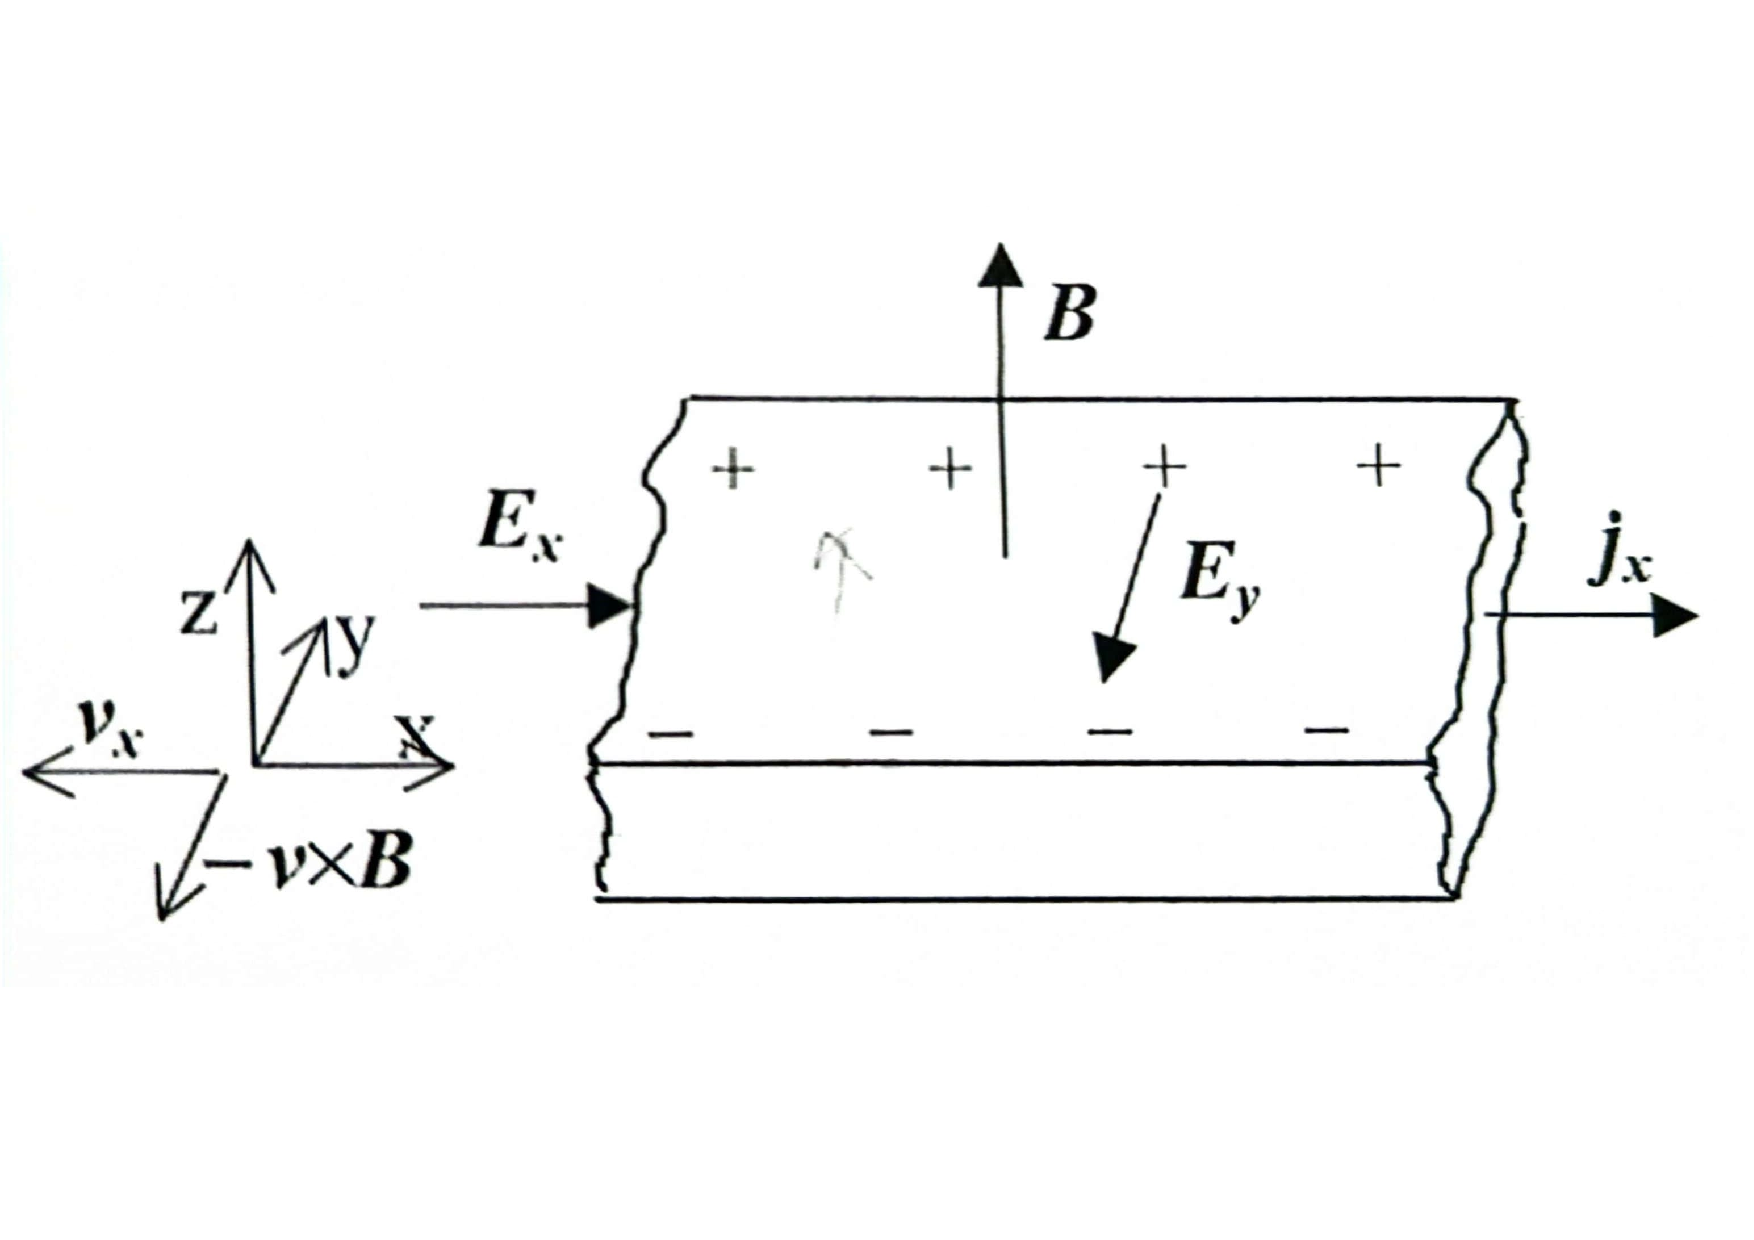
\includegraphics[scale=0.35]{Cuerpo/Ch_06/Fotos libro 7.pdf}
	\caption{Configuración experimental para comprobar el efecto Hall.}
	\label{Fig:06-07}
\end{figure}  

\begin{table}[h!] \centering
	\begin{tabular}{ccc c ccc}
		Metal & Valencia & $R_H^{\text{exp}}/R_H^{\text{teo}}$ & & Metal & Valencia & $R_H^{\text{exp}}/R_H^{\text{teo}}$ \\ \cline{1-3} \cline{5-7} 
		Li & 1 & 1.25 & & Na & 1 & 0.83 \\
		K & 1 & 0.83 & & Rb & 1 & 1.0 \\
		Cs & 1 & 1.1 & & Cu & 1 & 0.67 \\
		Ag & 1 & 0.77 & & Au & 1 & 0.67 \\
		Be & 2 & -5 & & Mg & 2 & -2.5 \\
		In & 3 & -3.3 & & Al & 3 & -3.3 
	\end{tabular}
	\caption{Coeficiente Hall de algunos elementos (relativos al resultado de la teoría de e$^-$ libres).}
	\label{Tab:06-03}
\end{table}



\subsection{Dependencia con la temperatura de la conductividad eléctrica}

Si admitimos que los dos mecanismmos de scattering principales (fonones y defectos) son independientes entre sí, la probabilidad de colisión por unidad de tiempo $\tau^{-1}$ será la suma de las debidas a ambos mecanismos por separado:

\begin{eqnarray}
	\tau^{-1} = \tau_{\text{def}}^{-1} +\tau_{\text{fon}}^{-1}
	\label{Ec:06-03-04}
\end{eqnarray}
Como los defectos estructurales en un cristal (impurezas qímicas, microgrietas, dislocaciones, etc.) no cambian esencialmente con la temperatura, dan una contribución a $\sigma$ constante. En cuanto a los fonones, la probabilidad de colisión variará porque, en particular, varía el número de aquellos. Así tenemos que para la resisitividad eléctrica $\rho\equiv 1/\sigma=m/ne^2 \tau$:

\begin{eqnarray}
	\rho = \rho_{\text{def}} + \rho_{\text{fon}} (T)
\end{eqnarray}
resultado que se conoce como la \textit{regla de Matthiesen}. A bajas temperaturas se tiene $\rho\approx \rho_{\text{def}}$, pues $\rho_{\text{fon}}(T)\rightarrow0$ al no existir fonones. En cristales ultrapuros y a muy bajas temperaturas $\tau$ o $\ell$ (y por tanto $\sigma$) pueden llegar a ser hasta 6 órdenes de magnitud mayores que a temperatura ambiente. A altas temperaturas, en el límite clásico ($T>\theta_{\text{Debye}}$) la distribución energética de los fonones cambia poco y lo que cuenta es su número medio. En particular , cabe esperar $\tau \propto \langle n \rangle_{\text{fon}}^{-1}$ y por tanto $\rho \propto \langle n \rangle_\text{fon}$. Como $\langle n \rangle_\text{fon} \propto T$ se predice la dependencia lineal de $\rho$ con $T$. Esto es en efecto lo que se encuentra experimentalmente en metales. En el caso de medios desordenados como aleaciones, metales amorfos, etc. predomina la dispersión electrónica por defectos sobre la dispersión por fonones y $\rho$ es casi constante.
\subsection{Conductividad AC y propiedades ópticas}

Se estudia en apartado la predicción del modelo de electrones libres para algunas de las magnitudes ópticas básicas como la reflectividad y la atenuación. Supóngase un campo electromagnético de frecuencia $\omega$ aplicado sobre el metal. Despreciando el efecto del campo magnético asociado y prescindiendo del carácter vectorial, la ecuación dinámica (\ref{Ec:06-03-02}), puede expresarse como $m\dot{v}=-mv/\tau-eE_0e^{-i\omega t}$. Probando para la velocidad media de portadores una solución de la forma $v=v_0 e^{i\omega t}$ (donde $v_0$ puede ser complejo para tener en cuenta posibles desfases) resulta $v=-e\tau E / m(1-i\omega\tau)$. Usando ahora $j=-nev$, se obtiene directamente $j=\sigma(\omega)E$ donde 

\begin{eqnarray}
	\sigma (\omega) = \frac{\sigma(0)}{1-i \omega \tau} \label{Ec:06-07-01}
\end{eqnarray}
Aquí $\sigma (0) = ne^2 \tau/m$ es la conductividad eléctrica para $\omega=0$, es decir, DC. Una primera consecuencia de (\ref{Ec:06-07-01}) es que cuando $\omega \tau \ll 1$, $\sigma (\omega) \approx \sigma (0)$, la corriente oscila a la misma frecuencia que $\Encal$, gracias a las colisiones, y el comportamiento es puramente resistivo. Sin embargo, cuando $\omega \tau \gg 1$ las colisiones no son lo suficientemente frecuentes para frenar la inercia de los electrones y éstos se retrasan con respecto a $\Encal$, diminuyendo la absorción de energía.

Aunque $\sigma (\omega)$ contiene en principio toda la respuesta del gas, es más conveniente utilizar la \textit{formulación óptica}, que consiste en usar permitividad eléctrica relativa $\varepsilon(\omega)$. Recuérdese que las ecuaciones de Maxwell conducen a la siguiente relación entre $\varepsilon (\omega)$ y $\sigma (\omega)$ 

\begin{eqnarray}
	\varepsilon (\omega) = 1 + \frac{i \sigma(\omega)}{\varepsilon_0 \omega} \label{Ec:06-07-02}
\end{eqnarray}
Al sustituir (\ref{Ec:06-07-01}) en (\ref{Ec:06-07-02}) se obtiene 

\begin{eqnarray}
	\varepsilon(\omega) = 1 + \frac{i \sigma_0 / \varepsilon_0 \omega}{1-i\omega \tau} \label{Ec:06-07-03}
\end{eqnarray}
Dos casos límite de (\ref{Ec:06-07-03}) son especialmente interesantes:

\begin{itemize}
	\item \textbf{Frecuencia bajas:} $\omega \tau \ll 1$ y $\omega \ll \sigma / \varepsilon_0$. Por ejemplo, en el cobre esto se cumple para $\omega/2\pi\ll 10^{12} \ \unit{\Hz}$ ($\lambda = 0.3\unit{\mm}$), que está en la frotera entre ondas muy cortas radio y el infrarrojo. En este límite (\ref{Ec:06-07-03}) queda 
	\begin{eqnarray}
		\varepsilon(\omega) = \frac{i\sigma_0}{\varepsilon_0 \omega}
	\end{eqnarray}
	Introduciendo el índice de refracción $n=\sqrt{\varepsilon(\omega)}=n_1 + i n_2$, y teniendo en cuenta $\sqrt{i}=(1+i)/\sqrt{2}$, resulta
	\begin{eqnarray}
		n = \sqrt{\frac{\sigma_0}{2\varepsilon_0\sigma}} (1+i) \label{Ec:06-07-05}
	\end{eqnarray}
	Al haber parte imaginaria habrá \textit{atenuación}: la amplitud del campo eléctrico se atenúe como $E\propto e^{ikx} \propto e^{\omega n_2 x/c} = e^{-x/2\delta}$ (se ha utilizado la relación de dispersión general de las ondas electromangéticas $\omega = ck /n$). La onda recorre una distancia $\delta$ antes de atenuarse, llamada \textit{profundidad de penetración}, que viene dada por 
	\begin{eqnarray}
		\delta = \sqrt{\frac{2\varepsilon_0 c^2}{\sigma_0 \omega}}
	\end{eqnarray}
	Por ejemplo para el cobre y con $\omega/2\pi \approx 10^{10} \unit{\Hz}$ (microondas $\lambda=3\unit{\cm}$) $\delta$ es tan sólo de unos $10 \ \unit{\um}$. En cuanto a la reflectividad 
	
	\begin{eqnarray}
		r = \left| \frac{n-1}{n+1} \right|^2 = \frac{(n_1-1)^2 + n_2^2}{(n_1+1)^2+n_2^2} \label{Ec:06-07-07}
	\end{eqnarray}
	Como, por (\ref{Ec:06-07-05}), $n_1 = n_2 = \sqrt{\sigma / 2\varepsilon_0 \omega} \gg 1$ (límite de bajas frecuenias), se tiene que $r\approx 1$, o sea, la reflectividad tiende al 100\%. De hecho es una regla general que cuanto más abosbe un material tanto más refleja en la superficie.
	
	\item \textbf{Frecuencias altas:} $\omega \tau \ll 1$. En este límite (\ref{Ec:06-07-03}) se aproxima por 
	\begin{eqnarray}
		\varepsilon (\omega) \approx 1 - \frac{\sigma_0 /\varepsilon_0 \tau}{\omega^2} = 1 - \frac{\omega_p^2}{\omega^2}
	\end{eqnarray}
	donde $\omega_p^2 = \sigma_0 / \varepsilon_0 \tau = ne^2 / \varepsilon_0 m$ se denomina \textit{frecuencia de plasma}. Se puede comprobar que $\omega_p$ corresponde a la frecuencia caractrística de oscilaciones longitudianles de la densidad de densidad del gas de electrones, cuyo \textit{cuanto} se denomina \textit{plasmón}. Estos modos de vibración electrónicas son muy energéticos corresponde al U.V. Para $\omega < \omega_p$, $\varepsilon(\omega)<0$, $n\approx n_2$ y existe atenuación. Asimismo, se ve en (\ref{Ec:06-07-07}) que $r \rightarrow 1$ al tender $n_1 \rightarrow 0$. Sin embargo, para $\omega > \omega_p$,$\varepsilon(\omega)$ es real, $n_2=0$ y el metal se hace \textit{transparente}. Esta transparenecia debe ocurrir en el U.V. Para algunos metales, como los alcalinos, esto se verifica bien. En general, las propiedes óptica de los metales son menos simples de los que predica el modelo de electrones libres y, de nuevo, la estructura de badndas es de referencia obligdaa para su explicación.
\end{itemize}

\section{Transporte térmico}

Drude, además de describir una ecuación que describe con cierta precisión la conductividad eléctrica, también fue suficientemente valiente como para calcular la conductividad térmica $\kappa_{el}$ debida a los electrones en movimiento\footnote{No hay que ignorar que la conductividad térmica tiene varias componentes, como la de los fonones $\kappa_{fon}$. En cualquier caso la predominante en la mayor parte de los metales es la procedente de los electrones.} usando la teoría cinética de Boltzmann. Como sabemos la conductividad térmica se define como la constante que relaciona un gradiente de temperatura y la corriente de calor $\jn_Q$:

\begin{equation}
	\jn_q = \kappa \nabla T
\end{equation}
La derivación usando la teoría de Boltzmann arroja que la la \textbf{conductividad térmica} $\kappa$ viene dada por

\begin{equation}
	\kappa = \frac{1}{3} n c_v \langle v \rangle  \ell
\end{equation}
donde $c_v$ es la capacidad calorífica por partícula, $\langle v \rangle $ es la velocidad promedio y $\ell = \langle v \rangle \tau$ es el \textit{recorrido libre medio} por parte del electrón. Una manera intuitiva de llegar a esta ecuación es la siguiente: una densidad de $n$ electrones es capaz  de transportar una cantidad de calor $c_v T$ a una velocidad $\langle v \rangle $ a lo largo de una distancia $\ell$. Como hemos visto la capacidad calorífica usando el modelo de gas de electrones libres:

\begin{equation*}
	c_v = k_B  \frac{\pi^2}{2}  \frac{ T}{T_F} 
\end{equation*}
y la velocidad promedio aproximable como la velocidad de Fermi $\langle v \rangle \approx v_f$, tenemos que la \textit{conductividad térmica} debida a los electrones viene dada por

\begin{equation}
	\kappa_{el} = \frac{\pi^2}{3} \frac{n \tau k_B^2 T}{m}
\end{equation}
Al igual que antes, esta cantidad viene dada por el parámetro desconocido $\tau$, al igual que la conductividad eléctrica. Entonces el cociente de ambas será una constante global (salvo por la temperatura) que no dependerá del metal. Entonces el \textbf{número de Lorentz} $L\equiv \kappa/\sigma T$ es una \textit{constante universal} tal que, según lo visto, viene dada por

\begin{equation}
	L = \frac{\kappa_{el}}{T \sigma} = \frac{\pi^2}{3} \frac{k_B^3}{e^2} \approx 2.45 \times 10^{-8} \unit{WattOhm/K^2}
\end{equation}
Este resultado fue considerado un éxito, y el hecho de que este ratio permanecía constante para casi todos los metales fue conocido durante mas de medio siglo como la \textbf{ley de Wiedemann-Franz}. 


\begin{table}[h!] \centering
	\begin{tabular}{ccc}
		Elemento & $L_{\text{exp}} (\unit{273 \kelvin})$ & $L_{\text{exp}} (\unit{373 \kelvin})$  \\
		& $10^8\unit{\watt \Omega / \kelvin^2}$ &  $10^8\unit{\watt \Omega / \kelvin^2}$ \\ \hline
		Ag & 2.31 & 2.37 \\
		Cu & 2.23 & 2.33 \\
		W  & 3.04 & 3.20 \\
		Zn & 2.31 & 2.33 \\
		Pt & 2.51 & 2.60
	\end{tabular}	
	\caption{Números de Lorentz experimentales para varios elementos.}
	\label{Tab:06-02}
\end{table}

\subsection{Efecto Peltier y Seebeck}

El \textbf{efecto Peltier} es el nombre que se le da la aparición de una corriente eléctrica $\jn$ cuando un metal o material tiene una corriente de calor $\jn_q$ no nula. El \textbf{coeficiente de Peltier} $\Pi$ viene dado como la constante que relaciona ambas corrientes:

\begin{equation}
	\jn_q = \Pi \jn
\end{equation}
Teniendo en cuenta que en la teoría cinética la corriente calorífica se define como

\begin{equation}
	\jn_q = \frac{1}{3} (c_v T) n \vn
\end{equation}
Usando que $\jn=-en\vn$ tenemos que el coeficiente Peltier vendrá dado entonces por:

\begin{equation}
	\Pi = - \frac{-c_v T}{3e}
\end{equation}
Otro coeficiente es el \textbf{coeficiente de Seebeck}, que describe otro fenómeno termoeléctrico, que es la formación de una fuerza termoeléctrica en un circuito cerrado que consta de dos metales diferentes, siempre que los puntos de contacto de estos metales estén a diferentes temperaturas. Denotado por $S$, se puede relacionar con el coeficiente Peltier a través de la relación $S=\Pi/T$, y viene dado por:

\begin{equation}
	S = \frac{c_V}{3e}
\end{equation}
según la teoría de Drude. 

\section{Interacción electrón-electrón}

En un metal la distancia media entre electrones de conducción es del orden de unos pocos $\unit{\angstrom}$ y, sin embargo, los recorridos libres medios para las colisiones electrón-electrón son mayores que $10^4 \unit{\angstrom}$ a temperatura ambiente, y superiores a 10 cm a 1 K. Uno de los factores responsables de esta falta de interacción entre electrones y que justifica la aproximación de electrones independientes es el Principio de Exclusión.

\begin{figure}[h!] \centering
	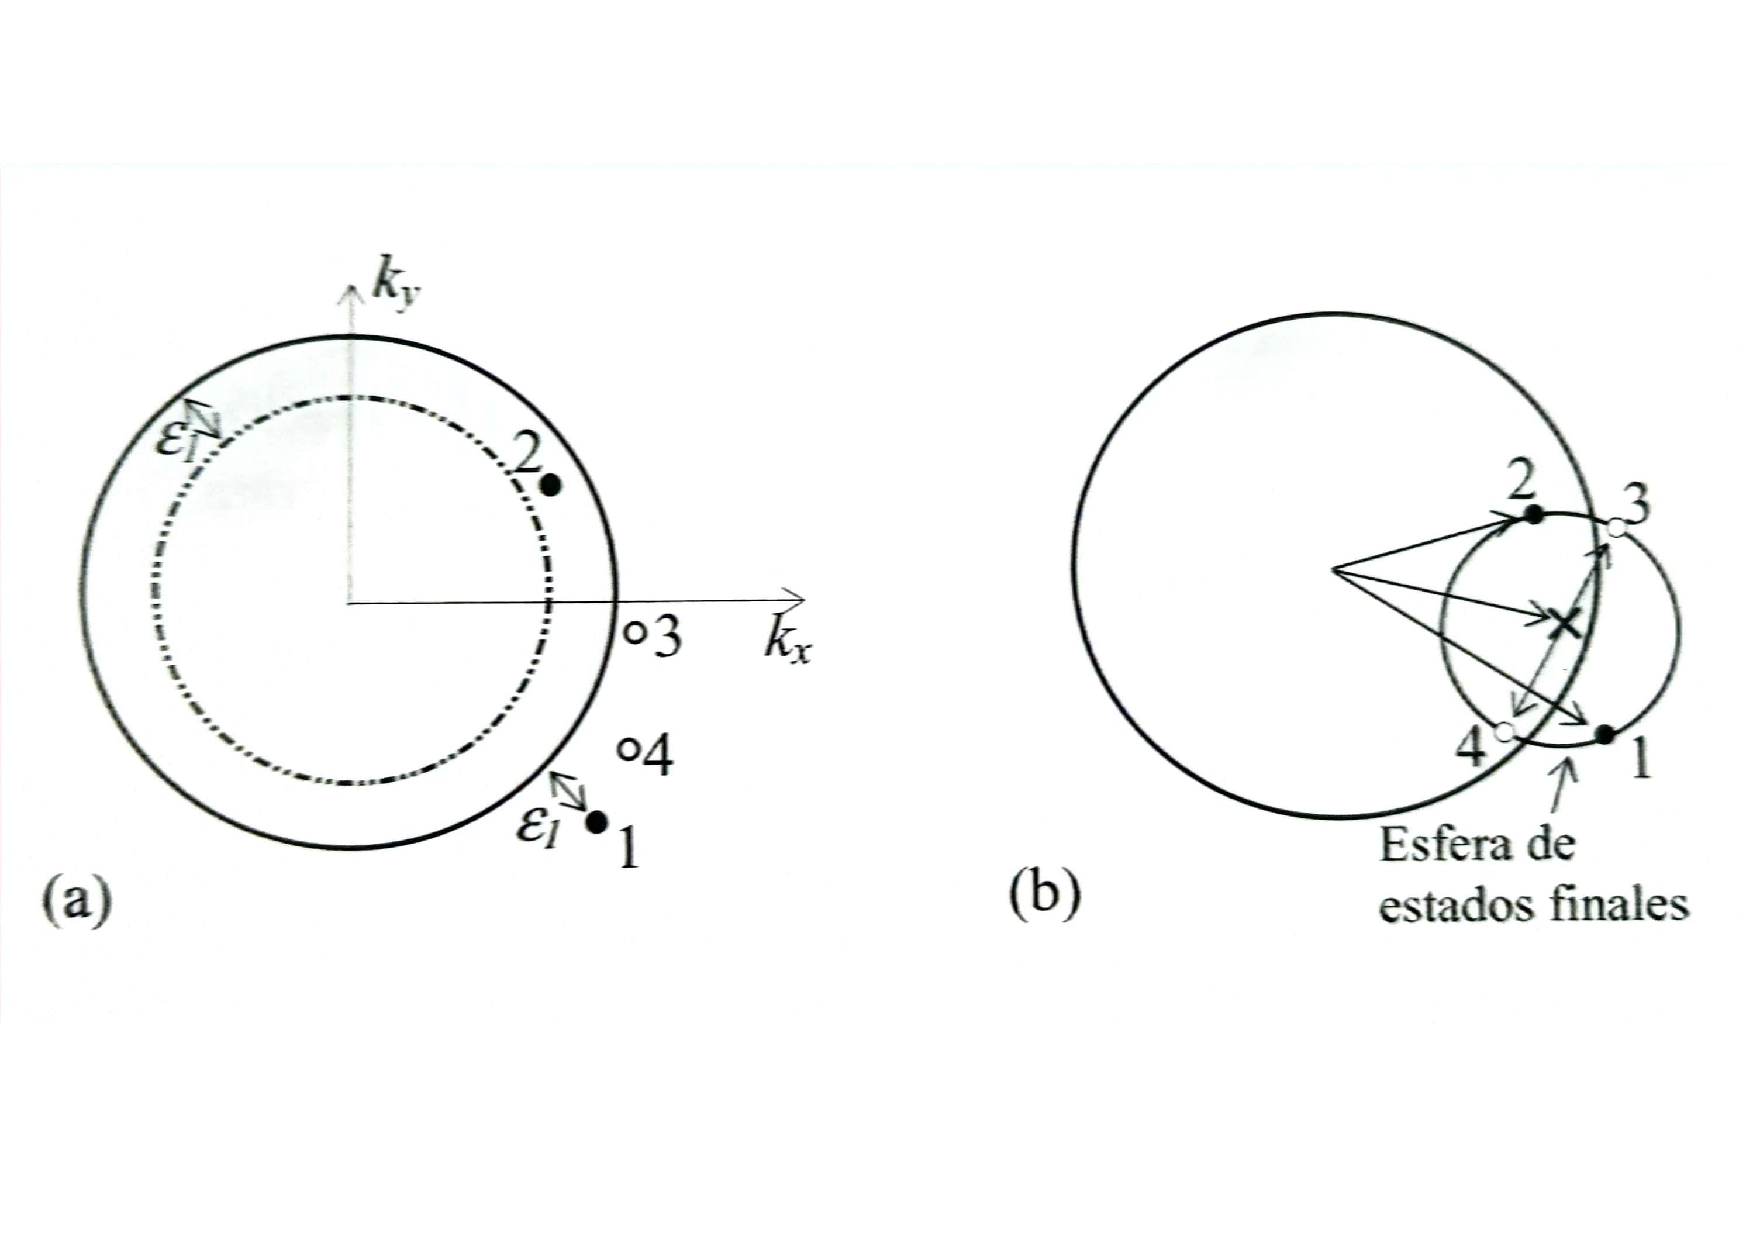
\includegraphics[scale=0.35]{Cuerpo/Ch_06/Fotos libro 4.pdf}
	\caption{Restricción a los procesos de colisión $e^- - e^-$ debido a las leyes de conservación de la energía (a) y del momento (b).}
	\label{Fig:06-04}
\end{figure}  

Consideremos la situación especialmente sencilla de una esfera de Fermi con un solo electrón excitado 1 con energía $\varepsilon_1$ respecto del nivel de Fermi. Como ilustra la figura \ref{Fig:06-04} (a), no todos los electrones 2 pueden colisionar con el 1, de modo que $1+2\rightarrow3+4$, pues los estados finales 3 y 4 deben estar desocupados. La condición $\varepsilon_3 + \varepsilon_4 = \varepsilon_1 + \varepsilon_2$ exige $|\varepsilon_2|<\varepsilon_1$ por lo que sólo una fracción $\sim \varepsilon_1 / \varepsilon_F$ de los electrones totales constituye un blanco para el electrón 1. La condición $\kn_1 + \kn_2 = \kn_3 + \kn_4$ limita aún más los estados finales: deben caer en la esfera de estados finales que ilustra la figura \ref{Fig:06-04} (b), y fuera del mar de Fermi la fracción permitida resulta ser también $\sim \varepsilon_1 / \varepsilon_F$. El producto de las dos fracciones es $\sim (\varepsilon_1/\varepsilon_F)^2$. 
En presencia de una temperatura finita puede equipararse $\varepsilon_1$ con $k_BT$, con lo que el Principio de Exclusión reduce las colisiones electrón-electrón en un factor $\sim (k_BT/\varepsilon_F)^2 \sim 10^4$. El correspondiente recorrido libre a temperatura ambiente es $\sim 10^4 \ \unit{\angstrom}$, mucho mayor que el debido a la interacción electrón-fonón.
